\documentclass[11pt,a4paper]{article}
\usepackage[utf8]{inputenc}
\usepackage[T1]{fontenc}
\usepackage[french]{babel}
\usepackage{lmodern}
\usepackage{geometry}
\usepackage{xcolor}
\usepackage{graphicx}
\usepackage{booktabs}
\usepackage{longtable}
\usepackage{hyperref}
\geometry{margin=2.1cm}
\hypersetup{colorlinks=true, linkcolor=blue, urlcolor=blue}
\title{\textbf{Script de présentation}\\Stéganographie LSB et détection automatique}
\date{12 juin 2026}

\begin{document}
\maketitle

\section*{Durée et logique}
Durée cible : 4 à 5 minutes. La slide 3 est réservée à la démonstration en direct.

Le fil logique est :
\begin{center}
\texttt{contexte du projet -> image RGB/LSB -> démonstration -> entraînement -> résultats}
\end{center}

\section{Slide 1 - Informations générales}
\textbf{Contenu :} ENSA Tanger, filière, titre complet, année universitaire, équipe projet et encadrant.

\textbf{Script oral :} Nous présentons un système de détection automatique de données dissimulées dans les images et vidéos numériques par analyse de texture et classification automatique. Le projet est réalisé à l'ENSA Tanger, filière Génie Cybersécurité et Cyberintelligence, année 2025-2026, par Zirar Chaimae, Fadili Nasrallah, Cheikh Mariam, Toukour Nouha et Oussafi Ilyas, encadrés par M. Ahmed Moussa.

\textbf{Transition :} Après le contexte, on explique le principe image-processing utilisé.

\section{Slide 2 - Principe image-processing}
\textbf{Contenu :} image RGB, séparation en canaux rouge/vert/bleu, plans LSB, extraction de caractéristiques.

\textbf{Script oral :} Une image RGB est une matrice de pixels. Chaque pixel contient trois valeurs : rouge, vert et bleu. Chaque valeur est codée sur 8 bits. La méthode LSB modifie le bit de poids faible. Cela change une valeur de 0 ou 1 seulement, donc la différence est presque invisible. En traitement d'images, on rend cette couche visible en séparant les canaux et en affichant les plans LSB.

\begin{figure}[h]
\centering
\begin{minipage}{0.31\linewidth}
\centering
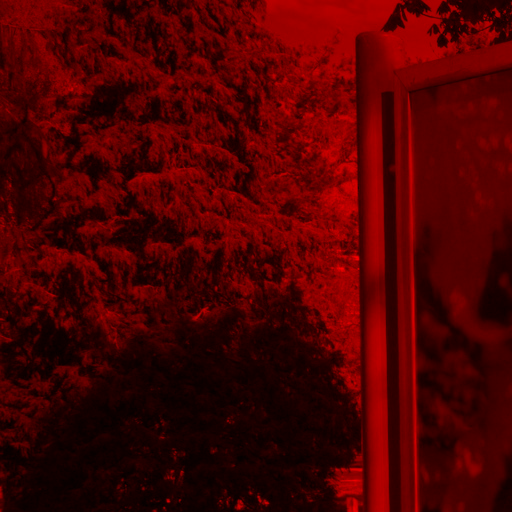
\includegraphics[width=\linewidth]{presentation_assets/canal_rouge.png}
\small Rouge
\end{minipage}
\hfill
\begin{minipage}{0.31\linewidth}
\centering
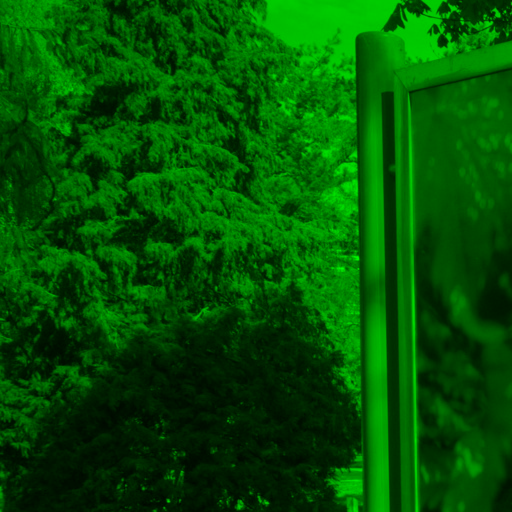
\includegraphics[width=\linewidth]{presentation_assets/canal_vert.png}
\small Vert
\end{minipage}
\hfill
\begin{minipage}{0.31\linewidth}
\centering
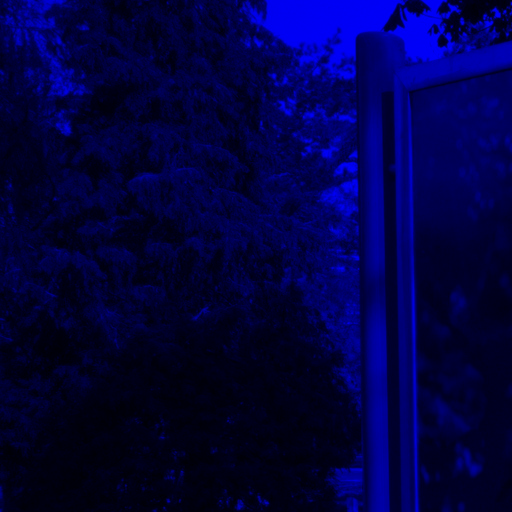
\includegraphics[width=\linewidth]{presentation_assets/canal_bleu.png}
\small Bleu
\end{minipage}

\vspace{0.25cm}

\begin{minipage}{0.31\linewidth}
\centering
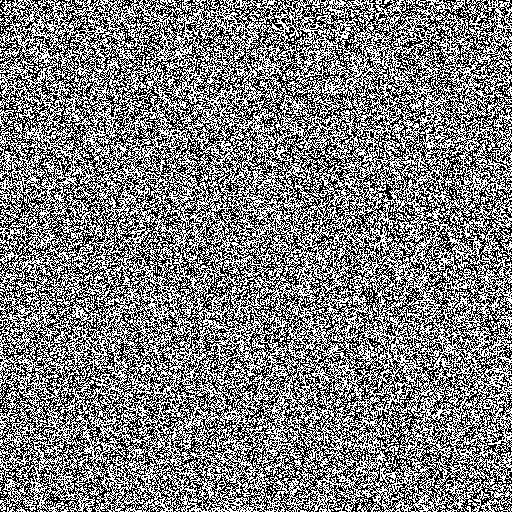
\includegraphics[width=\linewidth]{presentation_assets/lsb_rouge.png}
\small LSB rouge
\end{minipage}
\hfill
\begin{minipage}{0.31\linewidth}
\centering
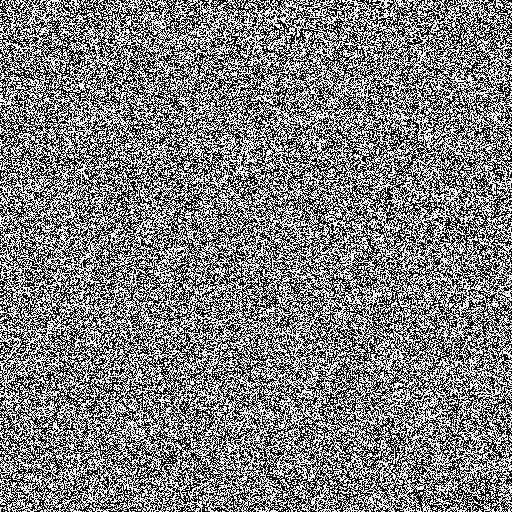
\includegraphics[width=\linewidth]{presentation_assets/lsb_vert.png}
\small LSB vert
\end{minipage}
\hfill
\begin{minipage}{0.31\linewidth}
\centering
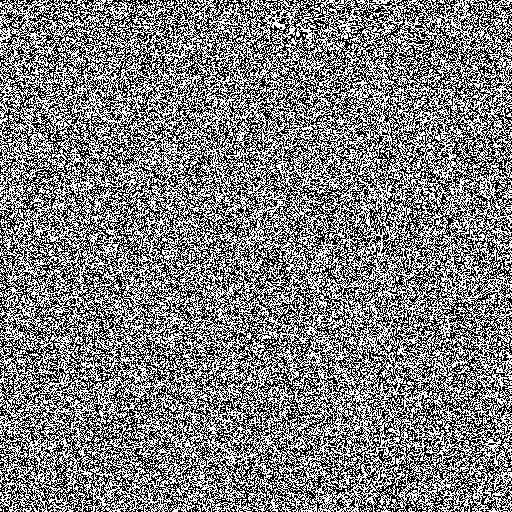
\includegraphics[width=\linewidth]{presentation_assets/lsb_bleu.png}
\small LSB bleu
\end{minipage}
\caption{Visuel à commenter : les canaux RGB gardent une structure visuelle, tandis que les plans LSB ressemblent à du bruit.}
\end{figure}

\textbf{Phrase importante :} Le verdict final ne vient pas d'une simple comparaison visuelle. Il vient de mesures calculées sur ces représentations : LSB, LBP, GLCM, histogrammes RGB et moments statistiques.

\clearpage

\section{Slide 3 - Démonstration en direct}
\textbf{Contenu :} cacher un message de 5 000 caractères, visualiser propre/stego/différence, détecter, extraire.

\textbf{Script oral :} Je choisis une image, puis j'insère un message UTF-8 de 5 000 caractères. L'application ajoute un en-tête de 32 bits qui contient la longueur du payload, puis écrit les bits du message dans les LSB des valeurs RGB. Ensuite, elle produit une image PNG pour éviter de perdre les bits à cause de la compression JPEG.

\begin{figure}[h]
\centering
\begin{minipage}{0.31\linewidth}
\centering
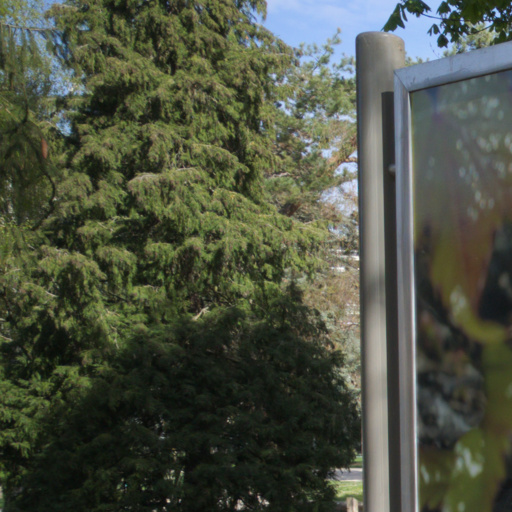
\includegraphics[width=\linewidth]{presentation_assets/demo_clean.png}
\small Image propre
\end{minipage}
\hfill
\begin{minipage}{0.31\linewidth}
\centering
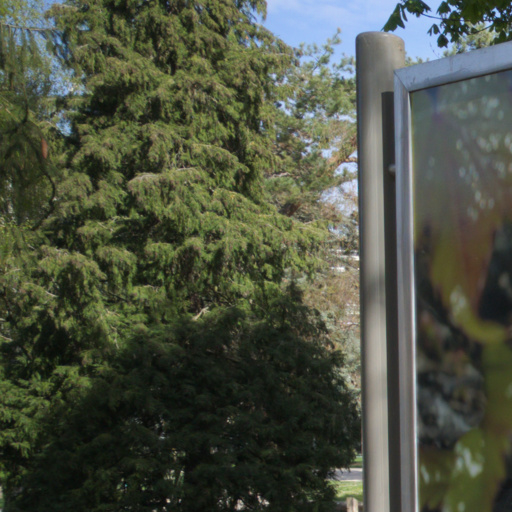
\includegraphics[width=\linewidth]{presentation_assets/demo_stego.png}
\small Image stego
\end{minipage}
\hfill
\begin{minipage}{0.31\linewidth}
\centering
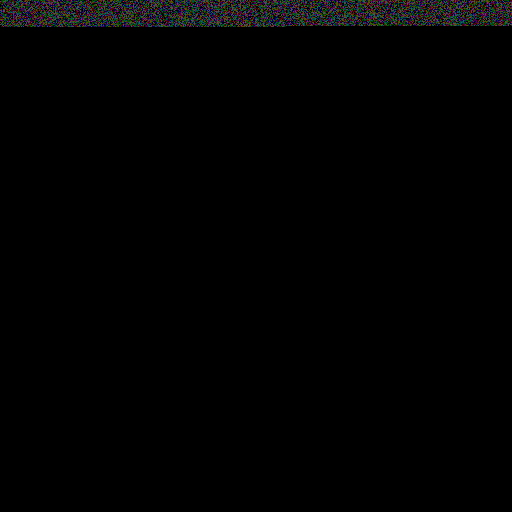
\includegraphics[width=\linewidth]{presentation_assets/difference_amplifiee.png}
\small Différence amplifiée
\end{minipage}
\caption{Visuel à commenter : l'image propre et l'image stego paraissent presque identiques, mais la différence amplifiée montre les valeurs modifiées.}
\end{figure}

\textbf{Données de la démonstration :} 20 359 valeurs RGB modifiées, PSNR environ 64 dB, extraction vérifiée de 5 000 caractères.

\textbf{Ordre à suivre :} Créer le PNG stego, le télécharger, le tester dans l'onglet Détection, puis l'ouvrir dans l'onglet Extraction.

\clearpage

\section{Slide 4 - Entraînement et modèles}
\textbf{Contenu :} dataset, génération des paires, split, features, modèles.

\textbf{Script oral :} Pour entraîner le système, nous avons utilisé 20 000 images cover ALASKA. Pour chaque image, nous avons créé une version propre PNG et une version stego PNG avec notre insertion LSB. Cette étape est importante : les deux classes ont le même format, donc le modèle ne peut pas apprendre simplement JPEG contre PNG.

Le split est fait par groupe. Une image source et sa version stego restent dans le même ensemble. Cela évite une fuite de données entre train et test. Ensuite, nous extrayons 218 caractéristiques par image : statistiques LSB, LBP, GLCM, histogrammes RGB et moments statistiques. Les modèles utilisés sont un SVM linéaire calibré et un Random Forest calibré.

\begin{figure}[h]
\centering
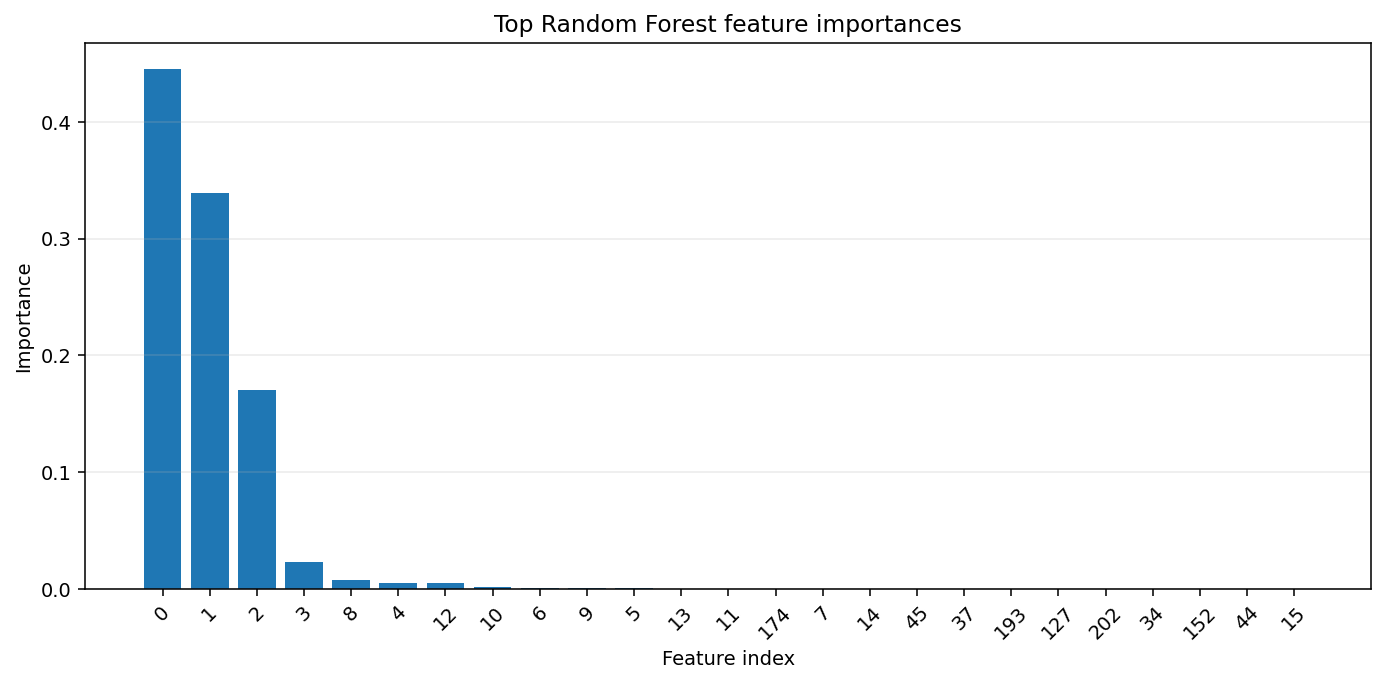
\includegraphics[width=0.72\linewidth]{results/feature_importance.png}
\caption{Visuel à commenter : le Random Forest permet de voir quelles familles de caractéristiques contribuent le plus à la décision.}
\end{figure}

\section{Slide 5 - Résultats et limites}
\textbf{Contenu :} métriques finales, matrices de confusion, limites du système.

\begin{longtable}{lrrrrrr}
\toprule
Modèle & Accuracy & Précision & Recall & F1 & AUC & Seuil \\
\midrule
SVM & 0.9983 & 0.9967 & 1.0000 & 0.9983 & 0.9995 & 0.5000 \\
Random Forest & 0.9983 & 0.9980 & 0.9987 & 0.9983 & 0.9999 & 0.7535 \\
\bottomrule
\end{longtable}

\begin{figure}[h]
\centering
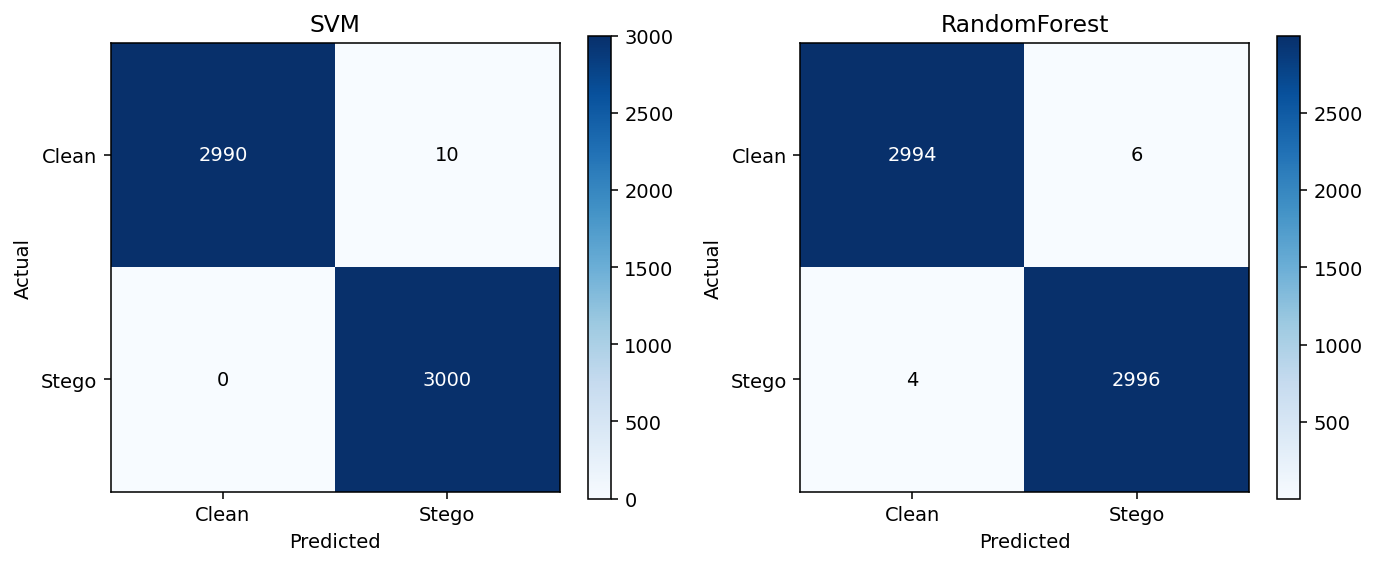
\includegraphics[width=0.72\linewidth]{results/confusion_matrices.png}
\caption{Visuel à commenter : les matrices de confusion montrent les bonnes classifications, les faux positifs et les faux négatifs.}
\end{figure}

\textbf{Script oral :} Les résultats sont très bons pour cette tâche précise : détecter notre stéganographie LSB sur les images ALASKA préparées. Il faut lire correctement ces résultats : ce n'est pas un détecteur universel de toutes les méthodes modernes comme JMiPOD, J-UNIWARD ou UERD. Le projet montre surtout le lien complet entre pixels, plans de bits, filtres de texture, statistiques et décision automatique.

\textbf{Phrase finale :} Une modification presque invisible devient détectable quand on observe les bonnes représentations de l'image.

\end{document}
